%!TEX root = "../../../DA_GUI.tex"

%	--------------------------------------------------------
% 	Debugger: Einleitung
%	--------------------------------------------------------

\section{Einleitung}

%   --------------------------------------------------------
%   Grundlegende Funktionen, Ideen
%   --------------------------------------------------------

\subsection{Die grundlegende Idee}
Ein wichtiger Bestandteil von C Compact ist der integrierte Debugger, der speziell für die Bedürfnisse von Anfängern ausgelegt ist. Während das Programm Schritt für Schritt abgearbeitet wird, sind alle Variablen und der Call Stack in übersichtlicher Form dargestellt. In der Variablentabelle werden Wertänderungen farbig hervorgehoben. Dadurch soll ein fundiertes Verständnis für den Programmablauf und die Logik dahinter entstehen.

\begin{figure}[htp]
\centering
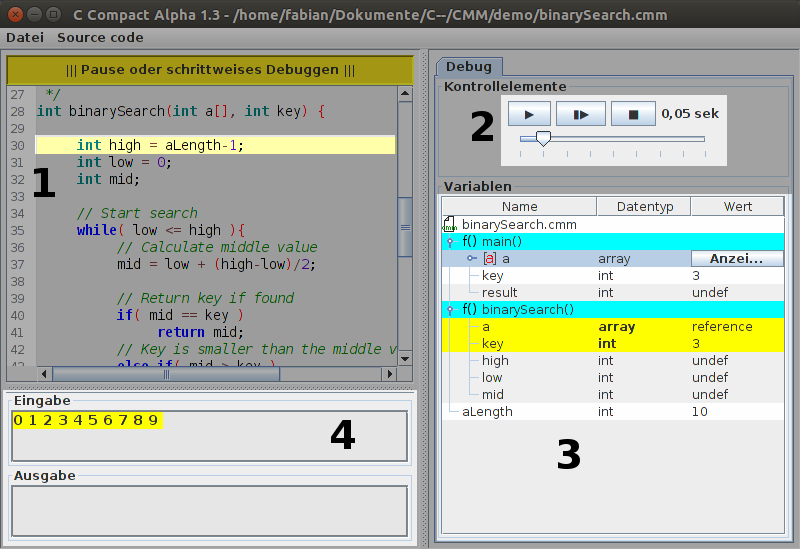
\includegraphics[width=0.7\textwidth]{./media/images/gui/debugger/gui-debugger-marked.png}
\caption{Die vier Komponenten des Debuggers}
\label{fig:deb-intro-m1}
\end{figure}

Während die Debugger professioneller Entwicklungsumgebungen eine Hilfestellung für erfahrene Programmierer sind, ist der Debugmodus von C Compact besonders auf Anfänger ausgelegt. Damit Einsteiger und unerfahrene Programmierer von Beginn an mit dem Debugger in Berührung kommen, ist er ein fester Bestandteil der Benutezroberfläche.

Abbildung \ref{fig:deb-intro-m1} zeigt die vier Komponenten des Debuggers in der Benutzeroberfläche:
\begin{enumerate}
\item Im Quelltext wird die gerade abgearbeitete Zeile markiert
\item Mit den Kontrollelementen kann der Debugger gestartet und angehalten werden
\item Die Variablen des Programmes werden übersichtlich angezeigt
\item Ein- und Ausgabe des laufenden Programmes befinden sich in getrennten Textfeldern, eingelesene Zeichen werden gelb markiert.
\end{enumerate}

%TODO somewhere else:
% Fehler im Präprozessor, Compiler oder Interpreter werden dem Benutzer übersichtlich angezeigt und verständlich erklärt. Außerdem werden Hinweise zur Fehlersuche und -behebung gegeben.
%TODO ref: nicht verwechseln mit internen Fehlern

%   --------------------------------------------------------
%   Bedienung des Debuggers
%   --------------------------------------------------------

\subsection{Bedienung des Debuggers}

Mit den Kontrollelementen kann der Debugger intuitiv und einfach bedient werden. Die Bedienelemente (Abbildung \ref{fig:deb-gui-ctrl}) sind im rechten Teil des Hauptfensters im Tab \glqq{}Debug\grqq{} (Siehe Kapitel \ref{sec:gui-main-right-reg-deb}) zu finden.

\def\arraystretch{1.4}
\begin{table}[h]
\begin{tabular}{|l|l|l|l|}
	\hline
	Element & \parbox{2cm}{Keyboard\\Shortcut}& Name & Funktion\\
	\hline
	\ding{228} / \ding{122}\thinspace \ding{122} & F5 & Play/Pause & Startet den Debugger/Hält den Debugger an\\
	\ding{122}\thinspace \ding{228} & F6 & Step & Springt zum nächsten Schritt weiter\\
	\ding{110} & F7 & Stop & Beendet den Debugger\\
	--- & --- & Schieberegler & \parbox{7cm}{Ändert die Zeitabstände beim automatischen Debuggen}\\
	\hline
\end{tabular}
\caption{Funktionen der Bedienelemente des Debuggers}\label{tab:deb-ctrl}
\end{table}



\begin{figure}[htp]
\centering
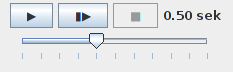
\includegraphics[width=0.4\textwidth]{./media/images/gui/debugger/ctrl-elements.png}
\caption{Kontrollelemente des Debuggers}
\label{fig:deb-gui-ctrl}
\end{figure}

Der Debugger hat vier unterschiedliche Modi, diese wurden bereits in Kapitel \ref{sec:gui-main-left-zust} überblicksmäßig beschrieben. Der Wechsel zwischen diesen Zuständen erfolgt durch Eingaben des Benutzers, entweder mit den Kontrollelementen (Buttons) in der Benutzeroberfläche, oder mit Keyboard Shortcuts.
%TODO ref keyboard shortcuts

Die vier Zustände sind:
\begin{enumerate}
\item \textbf{Text bearbeiten (ready mode)}
\item \textbf{Fehler aufgetreten (error mode)}
\item \textbf{Programm Schritt für Schritt abarbeiten oder Pause (pause mode)}
\item \textbf{Programm automatisch abarbeiten (run mode)}
\end{enumerate}

\begin{figure}[htp]
\centering
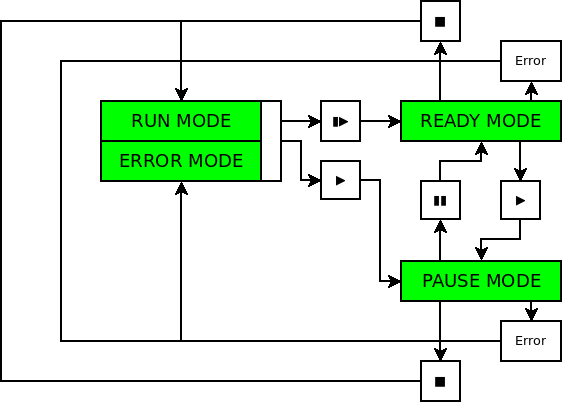
\includegraphics[width=0.65\textwidth]{/home/fabian/Dokumente/C--/CMM/doc/de/media/images/gui/debugger/RunModes_Simple.png}
\caption{Vereinfahctes Zustandsdiagramm des Debuggers}
\label{fig:deb-zust-simple}
\end{figure}

Obwohl der Debugger selbst zwischen Modus Editormodus (1) und Fehlermodus (2) unterscheidet, gibt es in der Benutzeroberfläche nur mehr den Editormodus. Der Fehlermodus wird trotzdem im Zustandspanel des Debuggers im Hauptfenster angezeigt, damit der Benutzer auf den aufgetretenen Fehler aufmerksam gemacht wird. Wie in Abbildung \ref{fig:deb-zust-simple} ersichtlich ist, erfüllen die beiden Modi die selben Funktionen.

Mit dem Schieberegler kann der Zeitabstand eingestellt werden, nach beim automatischen Debuggen zum nächsten Schritt gesprungen wird. Die gewählte Zeit wird, je nach zur Verfügung stehendem Platz, neben oder über dem Regler angezeigt.

\emph{Anmerkung 1:}
\par
\begingroup
\leftskip=1cm % Parameter anpassen
\noindent Der Pausemodus (3) hat zwei Funktionen: einerseits entspricht dieser Modus einer Pausierung (bezogen auf Zustand 4, in dem der Debugger automatisch durchläuft) und andererseits kann in diesem Modus mit dem mittleren Button auch direkt zum nächsten Schritt gesprungen werden.
\par
\endgroup


\emph{Anmerkung 2:}
\par
\begingroup
\leftskip=1cm % Parameter anpassen
\noindent Ein Sonderfall des run mode ist der \glqq{}quick run mode\grqq{}. Wenn der Regler für die Zeitabstände zwischen den Schritten des Debuggers auf null gestellt wird, werden die folgenden Schritte so schnell wie möglich abgearbeitet, bis entweder das Programm zu Ende ist oder der Debugger auf einen \glqq{}wait\grqq{}-Befehl stößt (Siehe Kapitel \ref{}).
\par
\endgroup
%TODO diesen Absatz nochmal lesen


%TODO bedienelemente können ausgeblendet werden

%TODO ref commands

%   --------------------------------------------------------
%   Schlüsselwörter
%   --------------------------------------------------------

\subsection{Schlüsselwörter}
%TODO ref compiler
%TODO ref panelRunListener
In der Sprache von C Compact gibt es zwei Schlüsselwörter, die zumindest im Endeffekt nicht vom Compiler oder Interpreter, sondern vom Debugger verarbeitet werden.

\subsubsection*{wait}
%TODO ref AST
Dieser Befehl kann an jeder beliebigen Stelle im Programm stehen. Der Compiler baut diesen Befehl als Element im Abstrakten Syntaxbaum ein. Wenn der Debugger diesen Knoten erhält, geht er in den Pause-Modus (3).

\subsubsection*{library}
Das Attribut \textbf{library} kann sowohl an einer Variable, als auch an einer Funktion angewandt werden. Das Schlüsselwort muss immer zwischen Typ und Name der Variable bzw. Funktion stehen.

Eine Variable mit dem \textbf{library}-Attribut wird im Debugger nicht angezeigt. Dies wird zum Beispiel verwendet, um die zahlreichen Konstanten der Bibliothek \textbf{math.h} im Debugger auszublenden.

Hat eine Funktion das \textbf{library}-Attribut, springt der Debugger nicht in diese Funktion, sondern arbeitet sie in einem Schritt ab. Dadurch können Bibliotheksfunktionen im Debugger wie einfache Befehle verwendet werden.
